
% ------------------------------% ------------------------------%
\chapter{Introduction}
%\addcontentsline{toc}{chapter}{Introduction}
%\markboth{Introduction}{Introduction}
% ------------------------------% ------------------------------%


Le point de départ des travaux exposés dans ce \modif{mémoire} est l'adoption par le Conseil de l'Europe, en octobre 2000, de la convention européenne du paysage. Ce traité invite chaque état signataire à considérer \modif{le paysage} comme un patrimoine commun. Il affirme l'utilité sociale de ce dernier pour le \modif{bien-être} individuel comme collectif et aborde sa place dans la qualité du cadre de vie, que \modif{celui-ci} soit urbain ou rural, remarquable ou anodin, préservé ou dégradé. 

La validation de la convention européenne du paysage par le Conseil de l'Europe s'est accompagné de la mise en place d’observatoires photographiques du paysage, afin de disposer d'un ensemble de données  permettant de réfléchir sur l'intégration du paysage dans les politiques d'aménagement du territoire. En France, ces observatoires prennent la forme de fonds photographiques numérisées, organisés en séries, chaque série étant rattachée à un point de vue geo-référencé qui est re-photographié régulièrement. Un protocole strict assure que les photographies d'une même série pourront être facilement comparées. Un intervalle de temps relativement long (quelques mois) sépare chaque prise de vue. 

\begin{figure}[h]
 \centering
	 \begin{subfigure}[t]{0.3\textwidth}	
			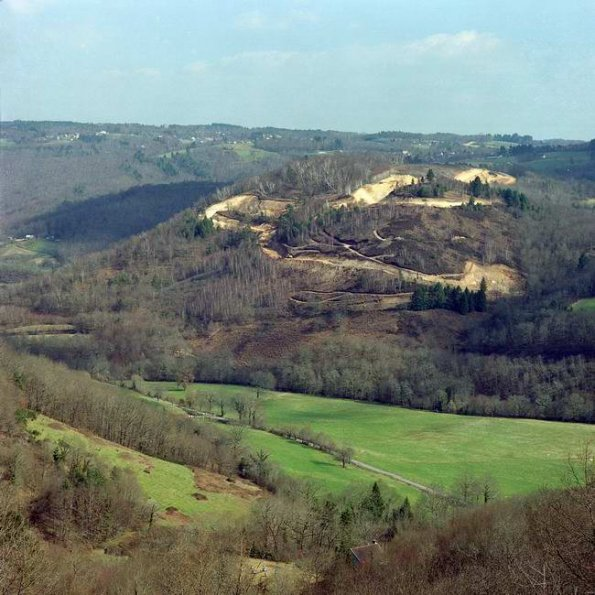
\includegraphics[width=\textwidth]{images/intro/opp_01}
	\end{subfigure}
	~
	 \begin{subfigure}[t]{0.3\textwidth}	
			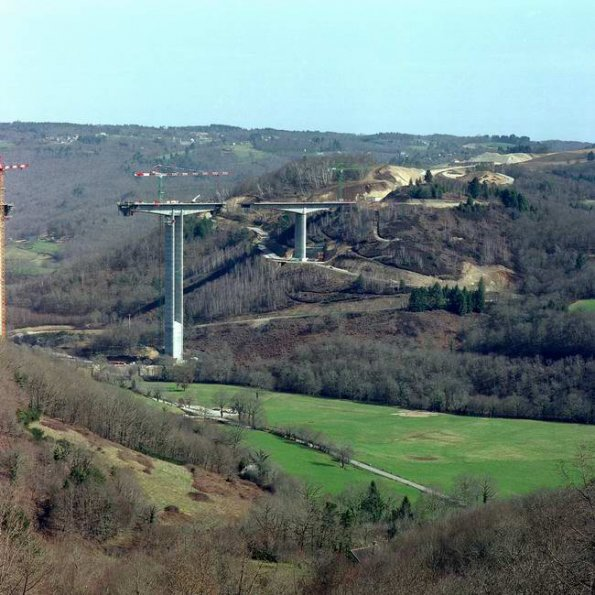
\includegraphics[width=\textwidth]{images/intro/opp_02}
	\end{subfigure}
	~
	 \begin{subfigure}[t]{0.3\textwidth}	
			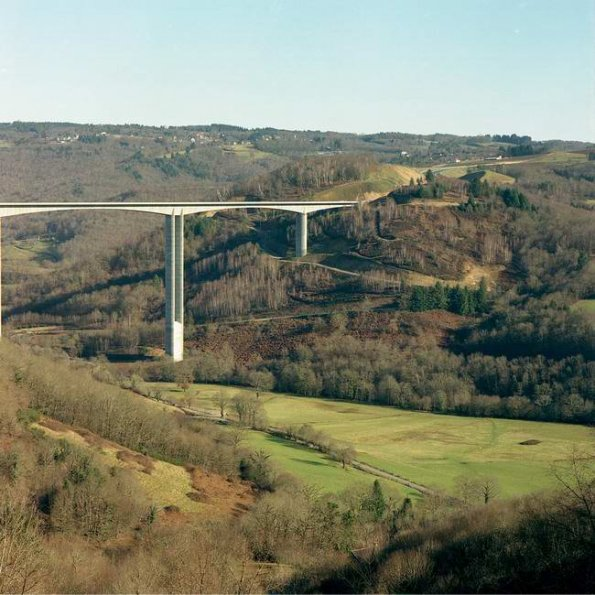
\includegraphics[width=\textwidth]{images/intro/opp_03}
	\end{subfigure}
	\caption{Photographie\modif{s} extraite\modif{s} de l'observatoire photographique du paysage mis en place lors \modif{de la construction} de l'autoroute A89.}
	\label{fig:intro:oppex}
\end{figure}

L'examen de ces fonds par des experts (géographes, personnes en charge de l'aménagement du territoire, etc.) permet d'analyser l'évolution d'un paysage lors d'un événement spécifique (construction d'un pont, chantier d'une \modif{autoroute}) ou d'étudier la dynamique de zones particulières (les territoires \modif{périurbains} par exemple). Leur mise à disposition pour le grand public participe à la valorisation du patrimoine \modif{paysager} et offre un outil aux citoyens pour s'impliquer davantage dans les actions publiques pouvant influencer \modif{leur} cadre de vie. 


La création, l'enrichissement et la consultation des données d'un observatoire photographique du paysage fait intervenir de nombreux outils informatiques. A minima, un observatoire photographique du paysage donne lieu à la mise en place d'un site web, par le biais duquel l'ensemble des citoyens peuvent accéder aux différentes séries de \modif{photographies}. La mise en place de traitements plus fins, capables d'extraire des informations pertinentes de ce catalogue d'images offrent de nombreux défis dans le domaine de la vision par ordinateur.

\section{Vision par ordinateur}
Olivier Faugeras \cite{faugeras1993three} définit la vision par ordinateur comme la discipline se focalisant  sur les quatre problèmes \modif{suivants} :

\begin{itemize}
\item quelles informations peuvent être extraites à partir des données enregistrées par un capteur visuel (caméra, appareil photographique, etc.)\modif{?}
\item comment ces informations sont-elle extraites ?
\item comment doivent-elles être représentées ? 
\item à quel point peuvent-elles être utilisées par un système robotique pour réaliser une tâche donnée ? 
\end{itemize}

Actuellement les applications \modif{de} ce domaine débordent largement de la robotique et la vision par ordinateur peut être vue comme la construction de modèles algorithmiques possédant des propriétés semblables à celle de la vision humaine. Ainsi, à l'aide \modif{d'un ensemble} de connaissances \textit{a priori}, l'enjeu consiste à fournir une interprétation de l'information contenu dans \modif{une ou plusieurs images}. Concrètement, il s'agit d'extraire des primitives visuelles de l'image, de proposer une représentation des connaissances et de mettre l'une et l'autre en correspondance afin de fournir une interprétation fiable  et rapide de la scène. 

Les problèmes classiques en vision par ordinateur sont, par exemple, les procédés de contrôle de pièce dans la robotique industrielle, la navigation pour les véhicules autonome\modif{s}, la détection d’événements, la modélisation 3D d'objets ou d'environnement\modif{s}, la reconnaissance d'objets, etc.


\section{Application dans le cadre des observatoires photographiques du paysage}

Dans le contexte des observatoires du paysage, \modif{le capteur visuel peut être un smartphone, un appareil photographique grand public ou un appareil photographique professionnel}. Les données obtenues sont  des photographies \modif{couleur de grande taille}. \modif{Ces images sont généralement de bonne qualité : elles sont peu bruitées et les objets qu'elles contiennent sont nets}. La figure \ref{fig:intro:oppex} montre \modif{trois} images extraites d'une même série.

Nos travaux concernent l'identification et la localisation des objets présents dans ces photographies. Nous souhaitons attribuer à chaque pixel un label indiquant \modif{la catégorie d'objet à laquelle} il appartient (ciel, herbe, route, etc.). Parce qu'ils permettent d'extraire les régions correspondant aux éléments d'une image et de leur attribuer une signification, les algorithmes visant à réaliser de tels traitements appartiennent au domaine de \emph{\modif{la} segmentation sémantique}. Les méthodes produites au sein de cette thématique de recherche peuvent être entièrement automatiques ou bien semi-automatique\modif{s}. 

Nous avons choisi de nous intéresser aux méthodes semi-automatique\modif{s}, dans la perspective de créer un outil permettant d'enrichir les données d'un observatoire photographique du paysage. \modif{Cet outil} intervient au sein d'une application plus complexe, capable de guider un utilisateur vers le point à re-photographier le plus proche puis de l'aider à reprendre une photographie à l'identique. Avant d'être envoyé à un serveur stockant les séries de photographies, cette dernière peut alors être segmentée de manière à ce que les éléments importants qu'elle contient soit documentés et localisés précisément dans l'image. 

Formulé différemment, nous cherchons un moyen  efficace de sélectionner chacun des objets visibles et de lui attribuer un label correspondant à des catégories sémantiques propres à l'observatoire. Ce type de logiciel est appelé \emph{outil de segmentation interactive}.


\section{Segmentation interactive }

Une méthode de segmentation interactive est un outil informatique capable de sélectionner un ou plusieurs objets au sein d'une image \modif{à partir d'indications données par un utilisateur}. Le domaine d'application le plus courant \modif{de ce type d'algorithme} est celui des logiciels de \modif{manipulation} d'images, dont les deux plus connus sont sans doute Gimp \footnote{\url{http://gimp.org}} et Photoshop \footnote{\url{http://www.photoshop.com}}. 

\begin{emodif}
Ce type d'algorithme se situe au croisement de deux thématiques : celle de la vision par ordinateur et celle de l'étude des interactions entre l'homme et la machine. 

Du point de vue de la vision par ordinateur, un accent particulier sera mis sur la formulation du problème de la segmentation interactive et sur les hypothèses qu'elle émet vis-à-vis du résultat recherché. Par exemple, certaines méthodes de segmentation interactive sont conçues pour extraire un unique objet du fond. Au contraire, d'autres algorithmes s'intéressent à la sélection simultanée de plusieurs objets, ce qui implique une augmentation significative de l'espace des solutions possibles. D'autres problématiques interviennent également de manière récurrente :  
\begin{itemize}
\item quelles primitives visuelles utiliser ? Par exemple, faut-il travailler directement au niveau du pixel ou rechercher des primitives visuelles plus complexes, telles que des groupes de pixels ? 
\item les indications données par l'utilisateur doivent-elles être considérées comme fiables ou faut-il envisager qu'elles contiennent des erreurs ? 
\item quel est le coût pour extraire un type d'information par rapport à son bénéfice dans la recherche d'un résultat ? Par exemple, si l'accès à la couleur d'un pixel est immédiat, analyser la texture présente dans son voisinage est une opération plus complexe, dont nous pouvons interroger la pertinence. 
\item est-il possible de trouver une solution exacte au problème posé ou faut-il se contenter d'une approximation ?
\item quelles approches permettent une recherche rapide de cette solution, qu'elle soit exacte ou approchée ?
\end{itemize}

L'étude des interactions entre l'utilisateur et le programme mettra l'accent sur l'ergonomie de la méthode de segmentation interactive, se demandant par exemple :
\begin{itemize}
\item quelles modalités permettent à l'utilisateur de donner les indications nécessaires à la méthode ? 
\item pour une  modalité donnée, quel est son degré de pénibilité ?
\item l'impact de ces indications sur le résultat obtenu est-il facilement prévisible par l'utilisateur ? 
\item est-il facile d'apprendre à se servir de la méthode proposée ?
\item le temps nécessaire à la méthode pour obtenir un résultat à partir des indications en permet-il une utilisation fluide ? 
\end{itemize}


\end{emodif}

 
\section{Problématique}

Le problème que nous cherchons à résoudre est le suivant : soit une photographie couleur et un ensemble de pixels attribués à différentes \modif{catégories} par un utilisateur ; comment associer de manière fiable et efficace chaque pixel de l'image à l'une des \modif{catégories demandées} par l'utilisateur et ce, de façon à ce que la segmentation sémantique produite soit cohérente tant vis-à-vis du \modif{contenu de l'image} que des indications fournies par l'utilisateur ? 


Nous ne souhaitons pas nous limiter aux seules photographies des observatoires du paysage et cherchons à concevoir un outil de segmentation interactive qui \modif{pourrait constituer} une amélioration intéressante \modif{par rapport à ceux} utilisés actuellement dans les logiciels de manipulation d'images. Ainsi, nous n'avons aucune connaissance \textit{a priori} sur le contenu des photographies ni sur les objets que l'utilisateur souhaitera sélectionner. En d'autre\modif{s} terme\modif{s}, seules les indications données par l'utilisateur permettent d'apprendre les \modif{caractéristiques des catégories d'objets}. Cet apprentissage est propre à chaque photographie et doit être recommencé pour chaque nouvelle image. 

\begin{emodif}
Nous ne nous donnons pas de limite sur le nombre d'objets à sélectionner et nous considérons que ce dernier varie d'une image à l'autre. Nous nous intéressons à la conception d'un algorithme itératif, où l'utilisateur peut corriger de manière intuitive les erreurs contenues dans le résultat obtenu, afin de converger rapidement vers la sélection qu'il désire. Nous supposons également que les indications données par l'utilisateur sont majoritairement fiables. 
\end{emodif}

Enfin, l'une des contraintes importantes de nos travaux concerne \modif{la rapidité} de la méthode que nous proposons. Dans le contexte des observatoires photographiques du paysage comme dans celui d'un logiciel de manipulation d'images, les photographies à traiter contiennent plusieurs millions de pixels. Le caractère interactif des algorithmes de segmentation interactive impose qu'un résultat soit fournit rapidement à l'utilisateur.  Notre choix des primitives visuelles et de la manière dont nous les utilisons doit garantir une faible complexité algorithmique.


\section{Organisation du mémoire}

Ce mémoire comprend sept chapitres.

\subsubsection*{\modif{Chapitre 1 -- Introduction --}} 
\modif{Nous présentons les motivations à l'origine des travaux décrits dans ce mémoire.}

\subsubsection*{\modif{Chapitre 2 -- Segmentation interactive --}} 
Nous présentons le domaine de la segmentation interactive et nous proposons une catégorisation des méthodes appartenant à cette \modif{thématique} : les méthodes de binarisation interactive par recherche des contours, les méthodes de binarisation interactive par recherche des régions \modif{et} les méthodes \modif{ de segmentation interactive multiclasse}. Pour chaque catégorie\modif{,} nous présentons quelques algorithmes de référence. 

\subsubsection*{\modif{Chapitre 3 -- Algorithme de segmentation interactive Superpixel $\alpha$-Fusion --}}
Nous proposons une nouvelle méthode de segmentation interactive \modif{multiclasse} $S \alpha F$, de l'anglais \og \emph{Superpixel $\alpha$-Fusion}\fg. Nous commençons par \modif{formuler} le problème de la segmentation interactive comme la minimisation d'une \modif{fonction de coût}. Cette fonction pouvant être factorisée, nous nous ramènerons à un problème d'optimisation dans un graphe de \modif{facteurs}. Un graphe de \modif{facteurs} est un graphe biparti où les sommets sont séparés en deux ensembles : les variables et les facteurs. \modif{Dans notre cas, les variables correspondent à de petits groupes connexes et homogènes de pixels : les superpixels}. Les facteurs correspondent aux sous-fonctions. Nous verrons comment les valeurs numériques de ces sous-fonctions peuvent être obtenues à l'aide d'une méthode de classification. 

\subsection*{\modif{Chapitre 4 --  Évaluation des méthodes de sur-segmentation --}}
Produire une sur-segmentation d'une image consiste à trouver une partition de ses pixels en petits ensembles connexes (les superpixels), dont la taille est nettement inférieure à celle des \modif{objets}. Pour la méthode que nous proposons, l'obtention d'une sur-segmentation est une étape clé. Nous avons donc réalisé une évaluation rigoureuse des algorithmes de sur-segmentation. Si la principale motivation de ce travail reste de sélectionner l'algorithme le plus approprié pour la méthode $S \alpha F$, les conclusions que permettent de tirer cette évaluation dépassent largement le cadre de la segmentation interactive.

\subsection*{\modif{Chapitre 5 -- Évaluation de l'algorithme $S \alpha F$ --}}

Ce chapitre concerne l'évaluation de $S \alpha F$. Nous comparons ses performances à celles des algorithmes de l'état de l'art \modif{décrits} dans le chapitre 2. Puis nous nous intéressons aux propriétés de \modif{$S \alpha F$}, notamment celles concernant son ergonomie. Nous concluons par deux applications de $S \alpha F$ : comme greffon pour le logiciel Gimp et comme outil d'annotation pour l'enrichissement d'un observatoire photographique du paysage.

\subsection*{\modif{Chapitre 6 -- Sur-segmentation adaptative par fusion de superpixels --} }

Nous terminons ce \modif{mémoire} par la proposition d'un nouvel algorithme de sur-segmentation, $ASARI$, de l'anglais \og \emph{\modif{Adaptive Superpixel Algorithm with Rich Information}}\fg . Ce dernier permet d'obtenir \modif{une} précision supérieure ou égale à celles des méthodes de l'état de l'art, avec un nombre \modif{inférieur} de superpixel\modif{s}. Par ailleurs\modif{,} les superpixels produits sont homogènes au sens de \modif{la} couleur et au sens de la texture. 

L'intégration de cet algorithme au sein de $S \alpha F$  constitue une perspective intéressante pour améliorer ses résultats. Elle requiert cependant :
\begin{itemize}
\item d'optimiser l'implémentation d'$ASARI$, les temps d'exécution de ce dernier étant encore trop important\modif{s} pour l'intégrer de manière bénéfique dans une méthode de segmentation interactive \modif{;} 
\item de réaliser des tests approfondis. L'une des particularités des superpixels produits par $ASARI$ étant d'intégrer une information de texture, au delà d'une simple évaluation montrant qu'$ASARI$ permet d'améliorer les performances de $S \alpha F$, il convient de vérifier si cette information de texture peut ou non avoir une influence positive sur la qualité des segmentations réalisées par $S \alpha F$.
\end{itemize}

Ces travaux restent à mener.


\subsubsection*{\modif{Chapitre 7 -- Conclusion -- }} 

\modif{Nous terminons par un résumé des contributions présentées et par quelques prolongements possibles de nos travaux.}